\chapter{Classifying Root Systems}
The classification of root systems can be found in several textbooks. \textcolor{red}{references !!!}

\section{Simple Roots}

For a particular root system $\Phi$ one may chose a subset (not neccesarily unique) of
roots called \textbf{simple roots} that are, in essence, building blocks of all the other roots
in the root system. \newline

For each root, $\alpha \in \Phi$, there exists a uniqe hyperplane passing through the origin that
is orthogonal to this root. Since the root system is only finite, the finite union of all
such hyperplanes can never be the whole ambient space, $E$. \newline

As such, it is always possible to find a vector $d \in E$ such that for any root $\alpha$, $\langle \alpha, d \rangle \not= 0$.
One partition the root system into two sets, $R^+(d)$ and $R^-(d)$, where $R^+(d) = \{
    \alpha \in \Phi |  <\langle \alpha, d \rangle > 0\}$ and $R^-(d) = -R^+(d)$. \newline

\begin{nameddefinition}{Simple Root}
    Let $d$ be a vector in a finite dimensional inner product space $E$, such that for any $\alpha$ in the root system, $\Phi$,
    $\langle \alpha, d \rangle \not= 0$. 
    If $\alpha$ belongs to $R^+(d)$ then it is a positive root, otherwise it is defined
    to be a negative root.
    A positive root is called \textbf{simple} if it is not the sum of any two other positive roots.
    The set of all such simple roots of a root system $\Phi$ is called a \textbf{basis} for $\Phi$.
\end{nameddefinition}

Fortunately, the choice of the vector $d$ above is not important.
Since the following remark is not directly related to the classification of root systems, it is only
discussed breifly, one can refer to the literature to learn more[\textcolor{red}{Weyl Groups and Chamber references}]. \newline

For every root $\alpha$ in a root system $\Phi$, there exists a hyperplace orthogonal to the root
and the union of all such hyplerplanes cut the ambient space $E$ into open, connected regions
called \textbf{Weyl Chambers}. \newline

Interestingly, one may construct a one-to-one correspondence between all bases
for a root systems and Weyl Chambers.

\textcolor{red}{Add lemma 1 and 2 from 3.1 and the bijection}


\section{Properties of Simple Roots}

We establish several useful lemmas that we use later.

\begin{lemma}
    \label{lemma:a-b}
    If the roots $\alpha, \beta$ in a root system $\Phi$ are not proportional and
    $\langle \alpha, \beta \rangle > 0$, then $\alpha - \beta \in \Phi$.
\end{lemma}

\begin{proof}
    It follows that $\langle \langle \alpha, \beta \rangle \rangle > 0$.
    Using Table \ref{table:enum}, we see that either $\langle \langle \alpha, \beta \rangle \rangle$ or 
    $\langle \langle \beta, \alpha \rangle \rangle$ is 1.
    If $\langle \langle \alpha, \beta \rangle \rangle$ is 1,
    then $\sigma_{\beta}(\alpha) = \alpha - \beta \in \Phi$.
    Otherwise, $\sigma_{\alpha}(-\beta) = \alpha - \beta \in \Phi$.
\end{proof}

\begin{lemma}
    \label{lemma:a.b_leq_0}
    Let $\alpha$ and $\beta$ be distinct simple roots in the root system $\Phi$,
    then $\langle \alpha, \beta \rangle \leq 0$.
\end{lemma}

\begin{proof}
    Assume to the contrary that $\langle \alpha, \beta \rangle \leq 0$.
    Then from the previous lemma (lemma \ref{lemma:a-b}),
    we know that $\gamma := \alpha - \beta \in \Phi\}$.
    If $\gamma$ is a positive root, then $\alpha = \gamma + \beta$ is also positive,
    contradicting our hypothesis. Otherwise, $-\gamma$ must be a positive root, in which case
    $\beta = \alpha + (-\gamma)$ is a positive root, yet again contradicting our hypothesis.
\end{proof}

\textcolor{red}{references !!!!}

The following lemma justifies the use of the term basis for the set of all simple roots.
\begin{lemma}
    \label{lemma:admit_config}
    The simple roots are linearly independent and span their ambient space.
\end{lemma}

And the proceeding lemma links the decomposability of a root system to its basis.
\begin{lemma}
    \label{lemma:decomp}
    A root system is decomposable if and only if its base is decomposable
\end{lemma}

\section{Classification of Root Systems}

From lemma \ref{lemma:a.b_leq_0}, we may deduce that for any two simple roots, the roots are either
orthogonal or the angle between them is obtuse. Much like the proof for the classification of Rank 2
Root Systems, from Table \ref{table:enum} we see that the angle between the aforementioned roots must
be either $\pi/2$, $2\pi/3$, $3\pi/4$ or $5\pi/6$. This information can be encoded into a graph. \newline

\begin{nameddefinition}{Coxeter Graph}
    The \textbf{Coxeter Graph} of a root system $\Phi$, is a (multi)graph, with each vertex
    corresponds to simple root of $\Phi$ and every pair of vertices $\hat\alpha, \hat\beta$ are
    connected by $\langle \langle \alpha, \beta \rangle \rangle \langle \langle \beta, \alpha \rangle \rangle = 
    4cos^2\theta$ edges, where $\theta$ is the angle between the simple roots $\alpha, \beta \in \Phi$
    corresponding to the vertices in the graph.
\end{nameddefinition}

Coxeter graphs do not however caprture all essential information about the simple roots of a root system.
In particular, the relative lengths of the roots (like when the angle between the roots is $3\pi/4$ or $5\pi/6$)
is not represented by the Coxeter Graph. \newline

\begin{nameddefinition}{Dynkin Diagram}
    A \textbf{Dynkin Diagram} of a root system is a Coxeter graph of the root system with arrows on
    the double or triple edges to indicate the shorter root
\end{nameddefinition}

In order to classify indecomposoable root systems it suffices to classify all possible Coxeter Graphs,
since the Dynkin Diagrams can be obtained from the Coxeter graphs by adding the arrows. \newline

\begin{nameddefinition}{Admissable Configuration}
    A linearly independent set of $n$ unit vectors $\{v_1, \dots, v_n \}$ that spans the ambient space
    $E$ is called an admissable configuration if for all $i\not=j, \langle v_i, v_j \rangle \leq 0$
    and $4 \langle v_i, v_j \rangle^2 \in \{0, 1, 2, 3\}$.
\end{nameddefinition}

Observe that the set of normalized simple roots of any root system is an admissable confifugration
by lemma \ref{lemma:admit_config}. \newline

\begin{nameddefinition}{Admissable Diagram}
    A Coxeter graph of an admissable configuration is called an admissable diagram
\end{nameddefinition}

From lemma \ref{lemma:decomp}, we know that the basis of an indecomposable root system cannot be
decomposed into mutually orthogonal subsets.
Therefore, the corresponding Coxter graph for an indecomposable root system will also be connected.
As such, to classify all indecompsable root systems it is sufficient to consider only connected
admissable diagrams.
This leads directly to the main classification theorem. \newline

\begin{namedtheorem}{Classification of Indecompsable Root Systems}
    The Dynkin Diagram of an indecomposable root system belongs to one of the nine families
    shown in Fig. \ref{img:dynkin}.
\end{namedtheorem}

\begin{figure}[h]
    \label{img:dynkin}
    \centering
    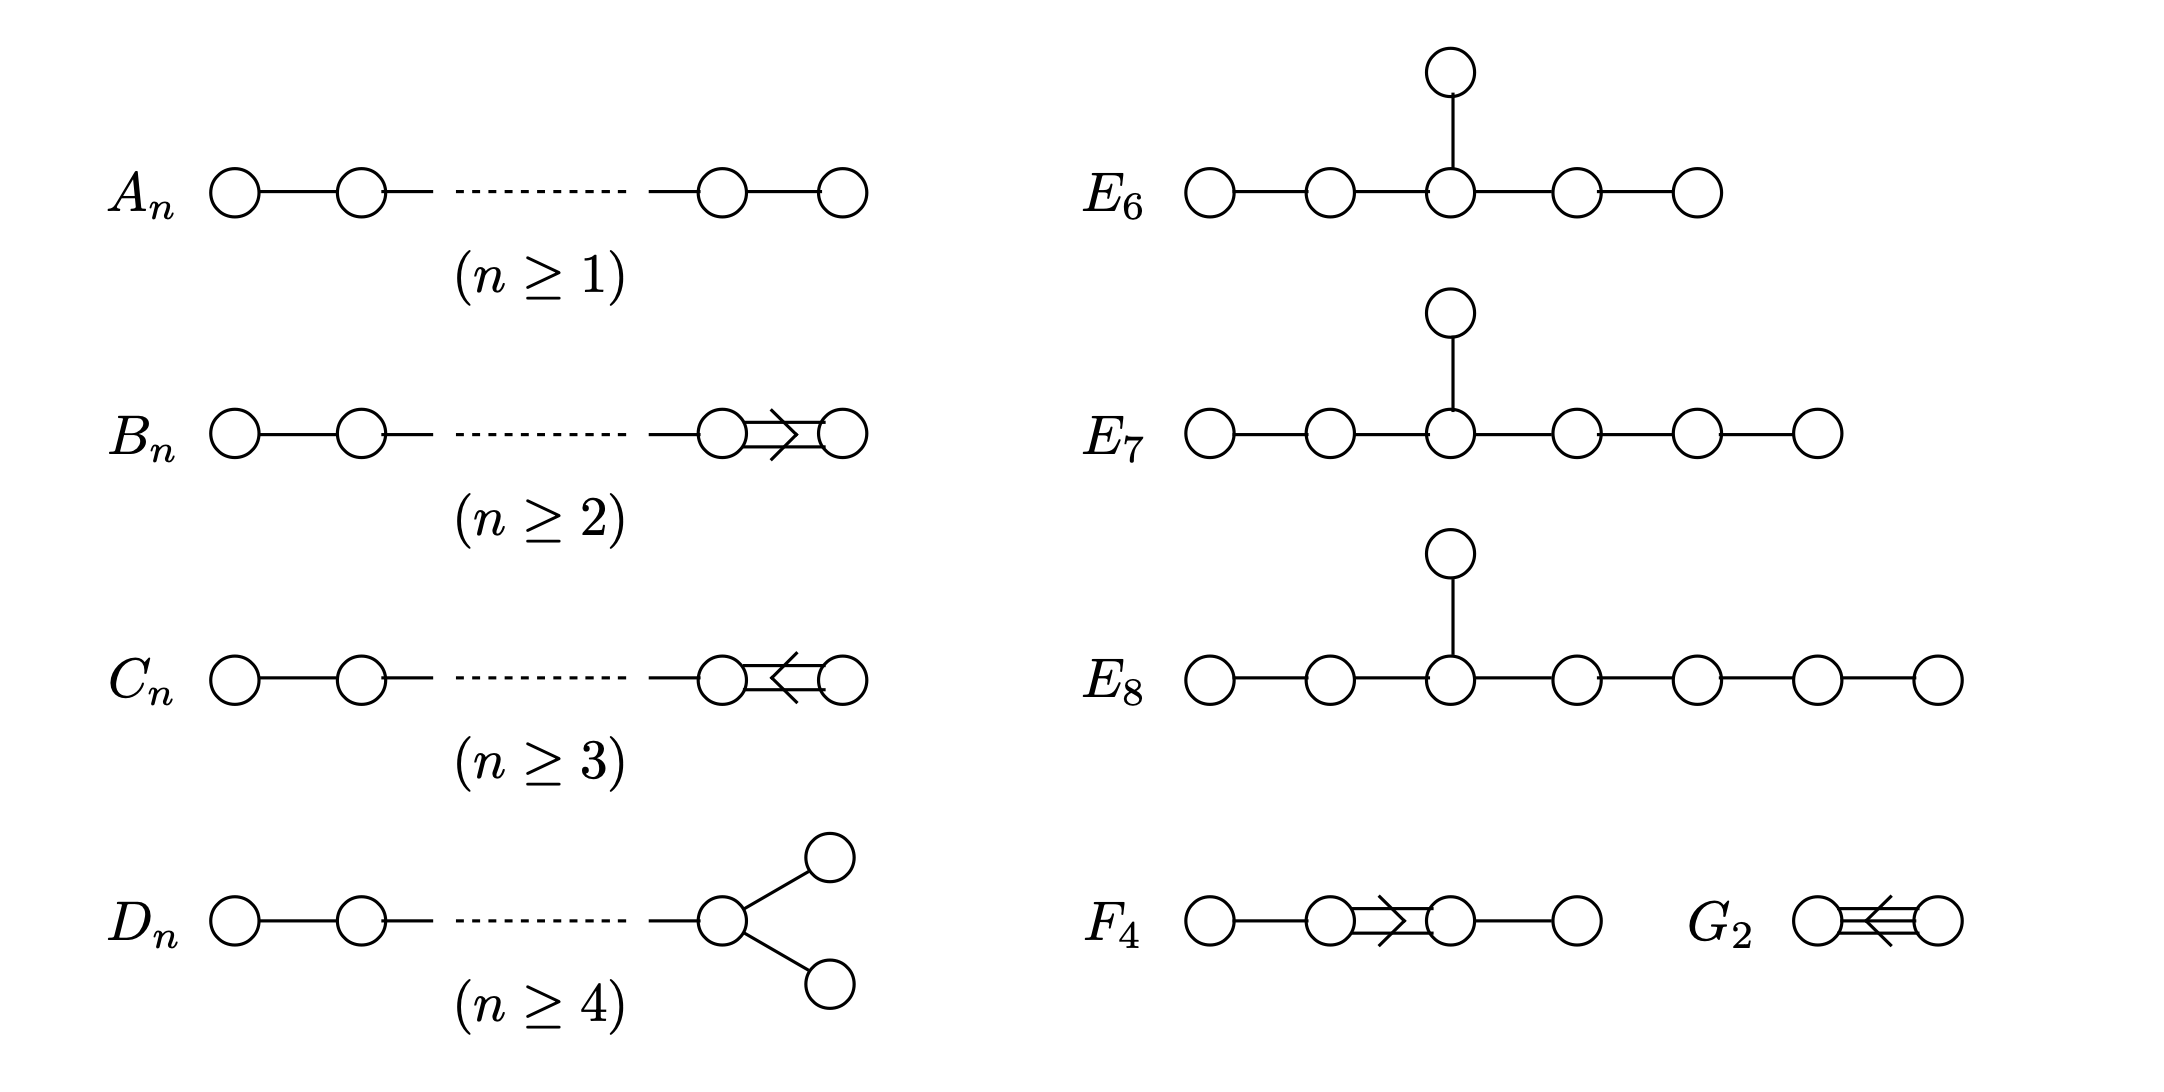
\includegraphics[scale=0.3]{./Dynkin.png}
    \caption{All possibilities for The Dynkin Diagram of Indecomposable Root Systems. Four infinite families and five exceptional root systems.}
\end{figure}

\begin{proof}
    We begin by classifying connected admissable diagrams and then proceeding to the Dynkin Diagrams. \newline
    
    Since the proof is large, it is split into the following steps.
    \begin{enumerate}
        \item Any subdiagram of an admissable diagram is also admissable. If the set 
        $\{v_1, \dots, v_n \}$ is an admissible configuration, then clearly any subset of it is also an admissible configuration
        (in the space it spans). The same holds for admissible diagrams.
        
        \item A connected admissable diagram is a tree. Let $v = \sum_{i=1}^{n} v_i$. Evidently, $v \not= 0$, since the admissable
        configuration is linearly independent. Then,
            \begin{equation*}
                0 < \langle v, v \rangle = v = \sum_{i=1}^{n} \langle v_i \rangle + \sum_{i < j} 2 \langle v_i, v_j \rangle = n + 2 \sum_{i < j} \langle v_i, v_j \rangle 
            \end{equation*}
            
        If the vertices $v_i$ and $v_j$ are connected, then $2 \langle v_i, v_j \rangle$ must take on a value in the set
        $\{-1, -\sqrt{2}, -\sqrt{3}\}$. In particular,  $2 \langle v_i, v_j \rangle \leq - 1$, hence the number of terms in the sum above
        cannot exceed $n-1$, so the number of distinct connected vertices must also be at most $n-1$. Since the diagram is connected,
        there must be at least $n-1$ such pairs. This leads to the conclusion that the number of distinct connected pairs of vertices
        is exaqctly $n-1$ and thus the diagram is a tree.
        
        \item No more than three edges (counting multiplicities) can originate from the same vertex.
        Let $c$ be any vertex (we refer to its corresponding root as $c$ as well when there is no ambiguity)
        and $\{v_1, \dots v_k \}$ be all vertices that are connected to $c$.
        Since the graph has no cycles, there are no edges between any $v_i$ and $v_j$.
        Therefore, $\langle v_i, v_j \rangle = 0$ when $i \not= j$ and $\{v_1, \dots v_k \}$ is an orthonormal set.
        Morevoer, since the simple roots are linearly independent, $c$ can not be expressed as a linear combination of $v_i$'s.
        Hence $c$ has a non-zero projection to the orthogonal complement of $\text{span}\{v_1, \dots v_k\}$.
        Normalize this projection and denote it by $v_0$.
        Then $\{v_0, v_1, \dots v_k \}$ is an orthonormal set and we can express $c$ as follows:
            \begin{equation*}
                c = \sum_{i=0}^k \langle c, v_i \rangle v_i
            \end{equation*}

        Since $c$ is a unit vector, $\langle c, c \rangle = \sum_{i=0}^k \langle c, v_i \rangle^2 = 1$. However 
        $\langle c, v_i \rangle^2 \not= 0$, thus,
            \begin{equation}
                \label{eq:l4}
                \sum_{i=1}^k 4\langle c, v_i \rangle^2 < 4
            \end{equation}
            
        Recall that the value $4\langle c, v_i \rangle^2$ denotes the number of edges between the vertices $c$ and $v_i$, hence
        it follows from equation \ref{eq:l4} that the number of edges originating from c are no more than 3.
            
        \item The only connected admissible diagram containing a triple edge is $G_2$ that is shown in Fig. \ref{img:dynkin}.
        This follows from the previous step. From now on we will consider only diagrams with single and double edges.
        
        Before proceeding any further, we recall the definition for a simple chain.
        \begin{definition}
            A \textbf{simple chain} in a graph is a non-repeating sequence of vertices such that every two consecutive vertices are
            connected with a single edge.
        \end{definition}

        \item Any simple chain $(v_1, ..., v_l)$ in a connected admissable diagram can be replaced by the single vector 
        $v = \sum_{i=1}^l v_i$. [See Fig \ref{img:collapse}]

        It suffices to show that $v$ is a unit vector and the new diagram obained after the replacement is connected and admissable.
        Note that,
            \begin{equation*}
                \langle v, v \rangle = l + \sum_{i < j} 2 \langle v_i, v_j \rangle
            \end{equation*}
        Since there are no cycles in the diagram, $\langle v_i, v_j \rangle = 0$ for all pairs where $i < j$ except for when $j = i+1$
        (i.e consecutive vertices). Then for consecutive verices, we have $\langle v_i, v_{i+1} \rangle = -1$, which is why 
        \begin{equation*}
            \sum_{i < j} 2 \langle v_i, v_j \rangle = \sum_{i  = 1}^{k-1} 2 \langle v_i, v_{i+1} \rangle = -(k-1)
        \end{equation*}
        And so $\langle v, v \rangle = 1$.

        Furthermore, since the diagram is acyclic, an arbitrary vertex $u$ not in the chain can be connected  to at most one vertex 
        (call it $v_m$) in the chain. Then,
            \begin{equation*}
                \langle u, v \rangle = \sum_{i=1}^{k} \langle u, v_i\rangle = \langle u, v_m \rangle
            \end{equation*}
        Consequently, when the whole chain is replaced by the single cevtor $v$, any vertex $u$ that was not in the chain reamains connected
        to $v$ in the same way it was to $v_m$. Hence, we can conclude that this new diagram is also connected and admissable.
        
        \begin{figure}
            \centering
            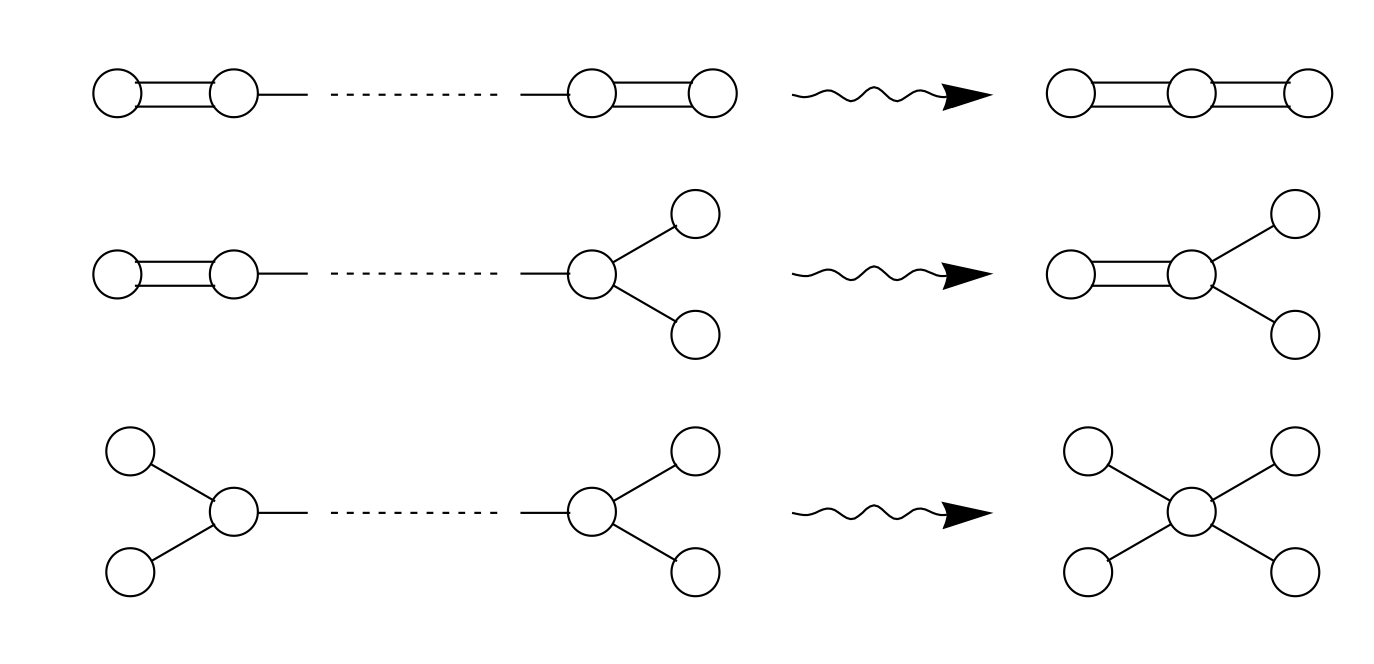
\includegraphics[scale=0.3]{./Dynkin_Collapse.png}
            \label{img:collapse}
            \caption{A Visualization of collapsing simple chains in step 5.}
        \end{figure}
    
        \item A connected admissible diagram has none of subdiagrams shown in Fig. \ref{img:collapse}.
        In each case the subdiagram contains a simple chain.
        According to Step 5 it can be collapsed to a single vertex. To the contrary, Step 3 shows that the obtained subdiagram is not
        valid, since it has a vertex of degree four. This contradiction Step 1.

        \item As such, a connected admissible diagram can contain at most one double edge and at most one branching, but not both
        of them simultaneously. Excluding, diagram G2 with a triple edge, we can make the following conclusion.
        There are only three possible types of connected admissible diagrams (see Fig. \ref{img:valid}):
        
        \begin{enumerate}[start=1,label={\bfseries T\arabic*:}]
            \item a simple chain
            \item a diagram with a double edge
            \item a diagram with branching
        \end{enumerate}
    
        \begin{figure}[h]
            \centering
            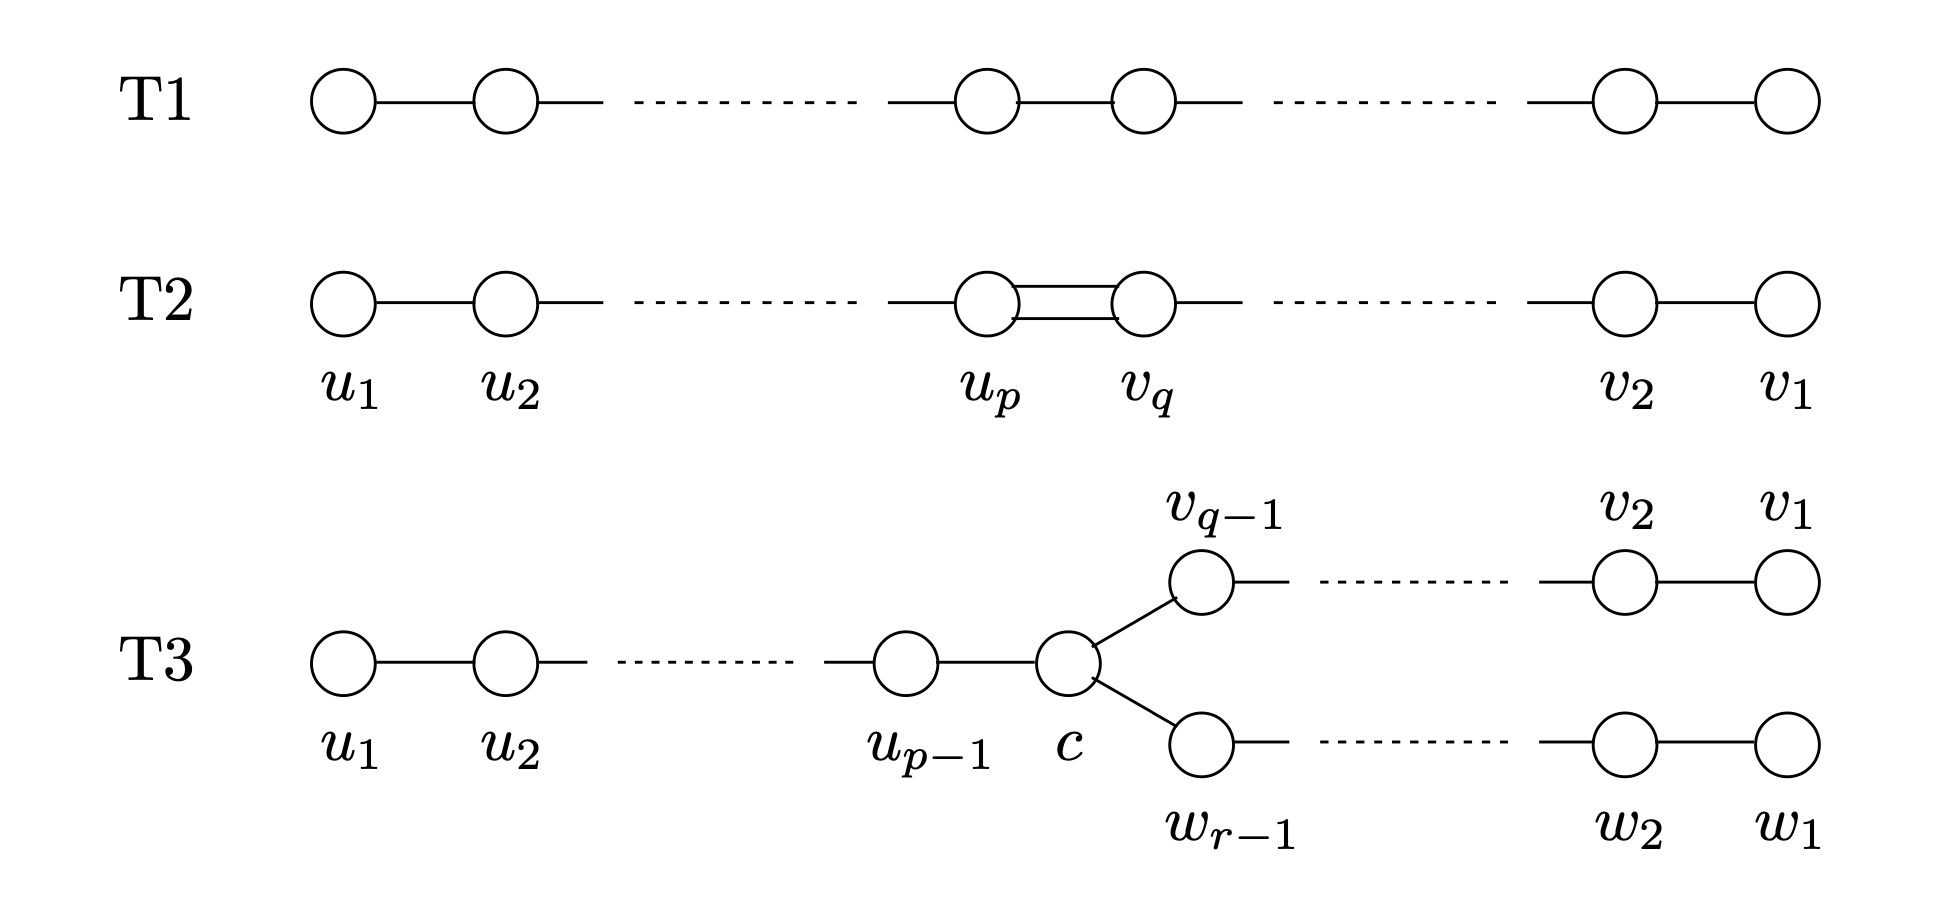
\includegraphics[scale=0.3]{./Dynkin_Valid.png}
            \caption{Possible types of connected admissable diagrams, excluding $G_2$.}
            \label{img:valid}
        \end{figure}

        \item The admissible diagram of type T1 corresponds to the Dynkin diagram $A_n$ in Fig. \ref{img:dynkin}, where $n \geq 1$.

        \item The only admissable diagrams of type T2 are $B_n \cong C_n$, and $F_4$. Define $u = \sum_{i=1}^{p} i \cdot u_i$, where $p$ is
        number of vertices before the double edge (See Figure \ref{img:valid}). A brief computation reveals,
        
        \begin{equation}
            \label{eq:self_inp}
            \langle u, u \rangle = \sum_{i=1}^p i^2 \langle u_i, u_i \rangle + \sum_{i < j} ij \cdot 2 \langle u_i, u_j \rangle
                = p^2 - \frac{p(p-1)}{2} = \frac{p(p+1)}{2}
        \end{equation}
    
        Likewise, define $v = \sum_{j=1}^q j \cdot v_j$ to get $\langle v, v \rangle = q(q+1)/2$.
        Then, $\langle u, v \rangle = pq \langle u_p , v_q \rangle$, since the double edge is the only edge between the components of
        $u$ and $v$. Then, $\langle u, v \rangle^2 = p^2q^2 / 2$ since the number of edges $4 \langle u_p, v_q \rangle$ is 2.

        Then, since $u$ is not a multiple of $v$ Cauchy-Schwarz holds strictly giving us,

        \begin{equation*}
            \frac{p^2q^2}{2} < \frac{p(p+1)}{2} \cdot \frac{q(q+1)}{2}
        \end{equation*}

        It is known that $p$ and $q$ are positive integers, so the only solutions are $p=1$ and $q$ is
        arbitrary (or vice versa) or $p = q = 2$. \newline

        The first solution corresponds to either of $B_n$ or $C_n$ (depending upon the choice of the short root), while the
        second solution corresponds to the Dynkin Diagram $F_4$ in Fig. \ref{img:dynkin}. \newline

        If $n=1$, both solutions correspond to $A_1$, however if $n=2$ then we have the case  for $B_2 = C_2$. Otherwise,
        we establish the convention that $B_n$ has $n \geq 2$ while $C_n$ has $n\geq 3$.

        
        \item Finally, we claim that the only admissable diagrams of type T3 are $D_n, E_6, E_7$ and $E_8$.
        As earlier, define $u = \sum_{i=1}^p i \cdot u_i$ and $v = \sum_{j=1}^q j \cdot v_j$. This time, also
        define $w = \sum_{k=1}^{r-1} k \cdot w_k$. Observe that there are no direct edges between the components 
        $u_i, v_j$ or $w_k$ so they exist in mutually orthogonal subspaces. This holds also for $u, v$ and $w$. \newline

        Using a similar argument to step 3, we can conclude that $c$ is not a linear combination of $u, v$ and $w$, hence:
        \begin{equation}
            \label{eq:cc_inp}
            1 = \langle c, c \rangle >  \langle c, \hat u \rangle^2 + \langle c, \hat v\rangle^2 + \langle c, \hat w \rangle^2
        \end{equation}
        where $\hat u, \hat v \text{ and } \hat w$ are the corresponding unit vectors for $u, v$ and $w$. So, 

        \begin{equation}
            \label{eq:cu}
            \langle c, \hat u \rangle^2 = \frac{\langle c, u \rangle^2}{\langle u, u \rangle}
        \end{equation}

        Note that no $u_i$ is connected to $c$ except for $u_{p-1}$, thus $ \langle c, u_i \rangle = 0$ for all $i \not= p-1$.
        Moreover, since they are connected by a single edge, $4 \langle c, u_{p-1} \rangle = 1$. Therefore, the numerator in
        the relation above (Eq. \ref{eq:cu}) is,

        \begin{equation*}
            \langle c, u \rangle ^2 = \sum_{i-1}^{p-1} i^2 \langle c, u_i \rangle^2 = (p-1)^2 \cdot \langle c, u_{p-1} \rangle = \frac{(p-1)^2}{4}
        \end{equation*}

        Whereas, the denominator (in Eq. \ref{eq:cu}) can be obtained to be $p(p-1) /2$ using Eq. \ref{eq:self_inp}. Then, 
        Eq. \ref{eq:cu} transforms into the following after some computation (note that $p \geq 2$).

        \begin{table}[h]
        \label{table:sol}
        \begin{center}
        \begin{tabular}{|| c | c | c | c ||}
            \hline $p$ & $q$ & $r$ & Dynkin Diagram\\ \hline
            any & 2 & 2 & $D_n$ \\ \hline
            3 & 3 & 2 & $E_6$ \\ \hline
            4 & 3 & 2 & $E_7$ \\ \hline
            5 & 3 & 2 & $E_8$ \\ \hline
        \end{tabular}
        \end{center}
        \caption{All possible integer solutions to inequality \ref{eq:ineq} and their corresponding Dynkin Diagrams of type T3.}
        \end{table}

        \begin{equation*}
            \langle c, \hat u \rangle^2 = \frac{1}{2} \left(1 - \frac{1}{p} \right)
        \end{equation*}

        Repeating this for $v$ and $w$ helps transform Eq. \ref{eq:cc_inp} into,

        \begin{equation}
            \label{eq:ineq}
            \frac{1}{p} + \frac{1}{q} + \frac{1}{r} > 1, \quad\quad p,q,r \geq 2
        \end{equation}

        Without loss of generaltiy, assume $p \geq q \geq r \geq 2$. Observe that $r < 3$ since the sum cannot exceed 1. This forces
        $r = 2$. If we take $q=2$ as well, then any feasible $p$ works. If $q=3$, however, then $p < 6$. No other solutions exist for
        $q \geq 4$. The correspondence between type T3 Dynkin Diagrams and the solution here are summarized in Table \ref{table:sol}.
    \end{enumerate}
    
    This completes the classification of all indecomposable root systems.

\end{proof}